% FEM 入门教程：为阅读 main.tex（FEM--DtN 富化误差估计讲义）准备的有限元基础
% 编译：latexmk -xelatex tutorial.tex
% 状态：draft
\documentclass[11pt,a4paper,fontset=fandol]{ctexart}
% Shared preamble for main.tex and tutorial.tex (load after \documentclass{ctexart}).
\usepackage[margin=2.5cm]{geometry}
\usepackage{amsmath,amssymb,amsthm,mathtools}
\usepackage{bm}
\usepackage{booktabs}
\usepackage{array}
\usepackage{graphicx}
\usepackage{caption}
\usepackage{subcaption}
\usepackage{enumitem}
\usepackage{tikz}
\usepackage{pgfplots}
\usepackage[numbers,sort&compress]{natbib}
\usepackage{hyperref}

\pgfplotsset{compat=1.18}
\usetikzlibrary{arrows.meta,decorations.pathreplacing,calc}
\hypersetup{colorlinks=true,linkcolor=blue!50!black,citecolor=blue!50!black,urlcolor=blue!50!black}
\captionsetup{font=small,labelfont=bf}
\setlength{\emergencystretch}{2em}
\setlist{itemsep=2pt,topsep=4pt}

\newcommand{\ii}{\mathrm{i}}
\newcommand{\ee}{\mathrm{e}}
\newcommand{\dd}{\mathrm{d}}
\newcommand{\RR}{\mathbb R}
\newcommand{\CC}{\mathbb C}
\newcommand{\nut}{\widetilde\nu}
\newcommand{\cell}{\mathcal C}

\theoremstyle{plain}
\newtheorem{proposition}{命题}
\newtheorem{lemma}{引理}
\newtheorem{theorem}{定理}
\theoremstyle{definition}
\newtheorem{assumption}{假设}
\newtheorem{example}{例}
\newtheorem{definition}{定义}
\theoremstyle{remark}
\newtheorem{remark}{注}

% A shaded box for "key takeaway" paragraphs.
\newenvironment{keypoint}{\par\medskip\noindent\begin{minipage}{\linewidth}\hrule\smallskip\noindent\textbf{要点：}}{\smallskip\hrule\end{minipage}\par\medskip}


\title{有限元方法入门：\\为周期波导导模计算准备的基础知识}
\author{}
\date{草稿，2026 年 10 月}

\begin{document}
\maketitle

\begin{abstract}
本教程是讲义《周期线缺陷波导导模特征值的 FEM--DtN 富化估计》（下称“主讲义”）的配套材料，面向没有系统学过有限元方法的读者。
我们只讲主讲义真正用到的内容：从偏微分方程到弱形式、Galerkin 方法与矩阵特征值问题、三角形上的高阶拉格朗日元、曲边单元与数值积分、矩阵组装与准周期约束、静态凝聚（Schur 补），以及几个线性代数工具（广义特征值问题、特征值导数公式、二次特征值问题与 QZ 分解、Stein 方程）。
每个概念都配一个能手算的小例子。读者需要的预备知识是多元微积分（Green 公式）和线性代数（矩阵、特征值、共轭转置）。
\end{abstract}

\tableofcontents

% ======================================================================
\section{从偏微分方程到弱形式}
\label{sec:weak}

有限元方法不直接处理微分方程本身，而是处理它的“弱形式”（又叫变分形式）。这一节说明弱形式是什么、为什么要用它，以及它如何自动处理材料界面和周期边界。

\subsection{一维例子}

考虑区间 $(0,1)$ 上的特征值问题
\begin{equation}
\label{eq:1d-strong}
-u''(x)=\mu\,u(x),\qquad u(0)=u(1)=0 .
\end{equation}
它的解是 $u=\sin(n\pi x)$，$\mu=(n\pi)^2$，$n=1,2,\dots$

取任意一个满足 $v(0)=v(1)=0$ 的光滑函数 $v$（称为\emph{测试函数}），把方程两边乘以 $v$ 再积分：
\[
-\int_0^1 u''v\,\dd x=\mu\int_0^1 u\,v\,\dd x .
\]
对左端分部积分：
\[
-\int_0^1 u''v\,\dd x=-\bigl[u'v\bigr]_0^1+\int_0^1u'v'\,\dd x=\int_0^1 u'v'\,\dd x ,
\]
边界项因为 $v(0)=v(1)=0$ 而消失。于是得到
\begin{equation}
\label{eq:1d-weak}
\int_0^1 u'v'\,\dd x=\mu\int_0^1 u\,v\,\dd x\qquad\text{对所有测试函数 }v .
\end{equation}
这就是弱形式。和 \eqref{eq:1d-strong} 相比，它有两个好处：
\begin{enumerate}
\item 它只用到 $u$ 的一阶导数。因此 $u$ 可以是“折线”这样只有一阶（分段）导数的函数，这正是有限元要用的函数类。
\item 方程对 $u$ 和 $v$ 是对称的。这会让离散后的矩阵是对称（复情形下是 Hermite）的。
\end{enumerate}
满足“函数及其一阶导数都平方可积”的函数构成的空间记为 $H^1$；若再要求边界值为零，记为 $H^1_0$。本教程对函数空间只需要这个直观理解。

\subsection{分段常数系数与界面条件}

现在设材料系数 $\rho(x)$ 在 $x=c$ 处跳跃：$x<c$ 时 $\rho=\rho_1$，$x>c$ 时 $\rho=\rho_2$。方程变为
\[
-u''=\mu\,\rho\,u\quad (x\ne c),
\]
物理上还要求界面条件：$u$ 与 $u'$ 在 $x=c$ 连续（电磁学中 TM 偏振正是这种情形）。

弱形式是什么？按同样的方法乘以 $v$ 积分，得到
\begin{equation}
\label{eq:1d-weak-rho}
\int_0^1 u'v'\,\dd x=\mu\int_0^1 \rho\,u\,v\,\dd x .
\end{equation}
材料系数只出现在右端的积分里，不需要单独处理界面。反过来看，弱形式自动蕴含了“$u'$ 连续”这一条件。为了看清这一点，设 $u$ 满足 \eqref{eq:1d-weak-rho}，并且在 $(0,c)$ 与 $(c,1)$ 上各自光滑。在两段上分别分部积分：
\[
\int_0^c u'v'=u'(c^-)v(c)-\int_0^c u''v,\qquad
\int_c^1 u'v'=-u'(c^+)v(c)-\int_c^1 u''v .
\]
代回 \eqref{eq:1d-weak-rho}，并利用两段上的方程 $-u''=\mu\rho u$，得到
\[
\bigl(u'(c^-)-u'(c^+)\bigr)\,v(c)=0\qquad\text{对所有 }v .
\]
取 $v(c)\ne0$ 即得 $u'(c^-)=u'(c^+)$。这类不需要写进函数空间、而由弱形式自动满足的条件叫做\emph{自然条件}。至于 $u$ 本身的连续性，它来自 $u\in H^1$：一维 $H^1$ 函数一定连续。

\begin{keypoint}
在弱形式中，材料系数只出现在积分里。界面上的导数连续条件是自然满足的，不需要特别处理。这也是为什么有限元网格不必严格贴合材料界面也能计算（只是精度会受影响，见主讲义第~5~节）。
\end{keypoint}

\subsection{二维情形与 Green 公式}

二维中分部积分换成 Green 公式。对区域 $D$ 及其外法向 $\bm n$，
\begin{equation}
\label{eq:green}
\int_D \nabla u\cdot\nabla w\,\dd x=-\int_D(\Delta u)\,w\,\dd x+\int_{\partial D}(\partial_{\bm n}u)\,w\,\dd s .
\end{equation}
它是散度定理 $\int_D\nabla\cdot\bm F=\int_{\partial D}\bm F\cdot\bm n$ 取 $\bm F=w\nabla u$ 的结果。

在我们的问题里，解是复值函数（下一小节会看到原因）。为了让 $\int|\nabla u|^2$ 这样的量出现，测试时乘以 $v$ 的\emph{复共轭} $\overline v$。方程 $-\Delta u=\mu\rho u$ 的弱形式于是写成
\begin{equation}
\label{eq:2d-weak}
\underbrace{\int\nabla u\cdot\nabla\overline v}_{=:a(u,v)}=\mu\underbrace{\int\rho\,u\,\overline v}_{=:b(u,v)} .
\end{equation}
这里引入的 $a(\cdot,\cdot)$ 和 $b(\cdot,\cdot)$ 分别叫\emph{刚度形式}和\emph{质量形式}（名字来自结构力学）。它们满足
\[
a(v,u)=\overline{a(u,v)},\qquad a(u,u)=\int|\nabla u|^2\ge0,\qquad b(u,u)=\int\rho|u|^2>0\ (u\ne0).
\]
若 $(\mu,u)$ 满足 \eqref{eq:2d-weak}，取 $v=u$ 得
\begin{equation}
\label{eq:rayleigh}
\mu=\frac{a(u,u)}{b(u,u)} ,
\end{equation}
所以 $\mu$ 是非负实数。右端称为 \emph{Rayleigh 商}。

\subsection{准周期边界条件}
\label{sec:qp-weak}

主讲义中的结构沿 $y$ 方向周期为 1。对这种问题，Floquet--Bloch 理论告诉我们：可以只考虑满足
\begin{equation}
\label{eq:qp}
u(x,y+1)=\ee^{\ii\beta}u(x,y)
\end{equation}
的解，其中 $\beta\in[-\pi,\pi)$ 是固定的 Bloch 参数。直观地说，平移一个周期，解只差一个相位因子。这样，问题就化为带状区域 $\{-1/2<y<1/2\}$ 上的问题，边界条件为
\[
u(x,\tfrac12)=\ee^{\ii\beta}u(x,-\tfrac12),\qquad \partial_yu(x,\tfrac12)=\ee^{\ii\beta}\partial_yu(x,-\tfrac12).
\]
$\beta\ne0$ 时 $u$ 一般是复值的。

在弱形式中，我们要求测试函数 $v$ 满足同样的值条件 $v(x,\tfrac12)=\ee^{\ii\beta}v(x,-\tfrac12)$。用 Green 公式时，上下两条边界上出现的边界项为
\[
\int\Bigl[\partial_yu(x,\tfrac12)\,\overline{v(x,\tfrac12)}-\partial_yu(x,-\tfrac12)\,\overline{v(x,-\tfrac12)}\Bigr]\dd x
\]
（下边界的外法向是 $-y$ 方向，故带负号）。代入两个条件：
\[
\partial_yu(x,\tfrac12)\,\overline{v(x,\tfrac12)}
=\ee^{\ii\beta}\partial_yu(x,-\tfrac12)\cdot\ee^{-\ii\beta}\,\overline{v(x,-\tfrac12)}
=\partial_yu(x,-\tfrac12)\,\overline{v(x,-\tfrac12)} ,
\]
两项正好相消。所以：
\begin{itemize}
\item 值的条件 $u(\cdot,\tfrac12)=\ee^{\ii\beta}u(\cdot,-\tfrac12)$ 要写进函数空间（称为\emph{本质条件}）；
\item 导数的条件是自然条件，由弱形式自动满足。
\end{itemize}
相消的关键是测试函数带了共轭：$\ee^{\ii\beta}$ 与 $\overline{\ee^{\ii\beta}}=\ee^{-\ii\beta}$ 相乘为 1。这也是测试时必须用 $\overline v$ 的原因之一。

\subsection{小结}

问题“求 $\mu$ 和 $u\ne0$ 使 $-\Delta u=\mu\rho u$，满足准周期条件”的弱形式是：在满足准周期值条件的 $H^1$ 函数空间 $V$ 中，求 $u\ne0$ 和 $\mu$，使得
\[
a(u,v)=\mu\,b(u,v)\qquad\text{对所有 }v\in V .
\]
材料界面条件和准周期导数条件都自动包含在内。

% ======================================================================
\section{Galerkin 方法：从弱形式到矩阵}
\label{sec:galerkin}

\subsection{有限维子空间与矩阵特征值问题}

弱形式中的空间 $V$ 是无限维的。Galerkin 方法的思想很简单：在一个有限维子空间 $V_h\subset V$ 中求解同样的方程。设 $V_h$ 的基为 $\psi_1,\dots,\psi_N$，写
\[
u_h=\sum_{j=1}^N c_j\psi_j ,
\]
并只用基函数作测试函数，$v=\psi_i$，$i=1,\dots,N$。代入弱形式：
\[
\sum_{j}a(\psi_j,\psi_i)\,c_j=\mu\sum_{j}b(\psi_j,\psi_i)\,c_j,\qquad i=1,\dots,N .
\]
定义 $N\times N$ 矩阵
\begin{equation}
\label{eq:KM}
K_{ij}=a(\psi_j,\psi_i)=\int\nabla\psi_j\cdot\nabla\overline{\psi_i},\qquad
M_{ij}=b(\psi_j,\psi_i)=\int\rho\,\psi_j\,\overline{\psi_i},
\end{equation}
分别叫\emph{刚度矩阵}与\emph{质量矩阵}，就得到广义矩阵特征值问题
\begin{equation}
\label{eq:Kc=muMc}
K\bm c=\mu M\bm c .
\end{equation}
由 \eqref{eq:KM} 和形式的性质，$K^*=K$，$M^*=M$（星号表示共轭转置），并且
\[
\bm c^*M\bm c=\int\rho\,|u_h|^2>0\quad(\bm c\ne0),\qquad \bm c^*K\bm c=\int|\nabla u_h|^2\ge0 .
\]
也就是说，$M$ 是 Hermite 正定矩阵。“系数向量的二次型等于对应函数的积分”这一事实在主讲义中会反复使用。

\subsection{一维例子：帽函数}
\label{sec:hat}

取 $(0,1)$ 的均匀剖分 $x_j=jh$，$h=1/(N+1)$。帽函数 $\psi_j$ 在 $x_j$ 处为 1，在其余节点为 0，在每个小区间上是线性的。它只在 $(x_{j-1},x_{j+1})$ 上非零，斜率为 $\pm1/h$。直接计算：
\[
K_{jj}=\int(\psi_j')^2=2\cdot\frac{1}{h^2}\cdot h=\frac2h,\qquad K_{j,j+1}=\int_{x_j}^{x_{j+1}}\Bigl(-\frac1h\Bigr)\Bigl(\frac1h\Bigr)=-\frac1h ,
\]
\[
M_{jj}=\int\psi_j^2=\frac{2h}{3},\qquad M_{j,j+1}=\int_{x_j}^{x_{j+1}}\psi_j\psi_{j+1}=\frac h6
\]
（取 $\rho=1$）。所以 $K=\frac1h\,\mathrm{tridiag}(-1,2,-1)$，$M=\frac h6\,\mathrm{tridiag}(1,4,1)$。

这两个矩阵的特征向量都是 $\bm c_j=\sin(n\pi x_j)$。记 $\theta=n\pi h$，利用 $\sin(a+\theta)+\sin(a-\theta)=2\sin a\cos\theta$，得
\[
K\bm c=\frac{2(1-\cos\theta)}{h}\,\bm c,\qquad M\bm c=\frac{h(2+\cos\theta)}{3}\,\bm c ,
\]
从而离散特征值为
\[
\mu_h=\frac{6}{h^2}\cdot\frac{1-\cos\theta}{2+\cos\theta} .
\]
用 $\cos\theta=1-\theta^2/2+\theta^4/24-\cdots$ 展开：
\[
\frac{1-\cos\theta}{2+\cos\theta}=\frac{\theta^2/2-\theta^4/24+\cdots}{3-\theta^2/2+\cdots}
=\frac{\theta^2}{6}\Bigl(1+\frac{\theta^2}{12}+\cdots\Bigr),
\]
于是
\[
\mu_h=(n\pi)^2\Bigl(1+\frac{(n\pi h)^2}{12}+O(h^4)\Bigr).
\]
特征值的相对误差是 $O(h^2)$。而折线逼近 $\sin(n\pi x)$ 时，导数的误差只有 $O(h)$。特征值误差大致是场（导数）误差的平方，下一小节解释原因。

\subsection{为什么特征值误差是场误差的平方}
\label{sec:square}

设 $(\mu,u)$ 是精确特征对，$w$ 是任意一个非零函数（例如近似特征函数），记 $e=w-u$。展开
\[
a(e,e)-\mu\,b(e,e)=\bigl[a(w,w)-\mu b(w,w)\bigr]-2\,\mathrm{Re}\bigl[a(u,w)-\mu b(u,w)\bigr]+\bigl[a(u,u)-\mu b(u,u)\bigr].
\]
由于 $u$ 满足弱形式，$a(u,v)=\mu b(u,v)$ 对任意 $v$ 成立（取 $v=w$ 与 $v=u$），后两个方括号都为零。两边除以 $b(w,w)$，得到
\begin{equation}
\label{eq:rq-error}
\frac{a(w,w)}{b(w,w)}-\mu=\frac{a(e,e)-\mu\,b(e,e)}{b(w,w)} .
\end{equation}
左边是 Rayleigh 商与精确特征值之差，右边是误差 $e$ 的二次式。离散特征值 $\mu_h$ 正是离散特征向量 $u_h$ 的 Rayleigh 商，所以 $\mu_h-\mu$ 与 $\|e\|^2$ 同阶。

这一性质是主讲义采用“比较不同精度下的特征值”这一思路的根本原因：特征值对场误差很不敏感，所以它比场本身收敛得快得多，层与层之间的差可以分辨得很精细。

\begin{remark}
对有界区域上的问题，由特征值的极小极大原理可以证明，Galerkin 特征值总是从上方逼近精确特征值。对最小特征值，这也可以直接从 \eqref{eq:rq-error} 看出：此时对任何 $e$ 都有 $a(e,e)\ge\mu\,b(e,e)$，右端非负。主讲义中的导模特征值位于本质谱的间隙中，右端的符号不再确定，离散特征值可能从任一侧逼近，也可能出现不对应任何真实特征值的“伪特征值”（称为谱污染）。这正是主讲义需要“饱和性假设”的原因之一。
\end{remark}

% ======================================================================
\section{三角形上的拉格朗日元}
\label{sec:lagrange}

有限元方法的“有限元”指的是：把区域剖分为许多小单元（这里是三角形），在每个单元上用多项式，并让它们在单元之间连续拼接。这一节讲如何在三角形上构造 $p$ 次多项式基函数。

\subsection{参考三角形与重心坐标}

\emph{参考三角形} $\widehat K$ 是顶点为 $(0,0)$、$(1,0)$、$(0,1)$ 的三角形，坐标记为 $(\xi,\eta)$。它的三个\emph{重心坐标}定义为
\[
\lambda_1=1-\xi-\eta,\qquad\lambda_2=\xi,\qquad\lambda_3=\eta .
\]
它们满足 $\lambda_1+\lambda_2+\lambda_3=1$；在三角形内部都非负；$\lambda_i$ 在第 $i$ 个顶点为 1，在对边上为 0。第~\ref{sec:mapping}~节会把参考三角形映射到实际的（可能是曲边的）单元上，所以只需在参考三角形上定义基函数。

\subsection{一次元与二次元}

一次（$P_1$）元：三个节点就是三个顶点，三个基函数就是 $\lambda_1,\lambda_2,\lambda_3$。

二次（$P_2$）元：六个节点为三个顶点和三条边的中点。基函数为
\[
\lambda_i(2\lambda_i-1)\quad(\text{顶点 }i),\qquad 4\lambda_i\lambda_j\quad(\text{顶点 }i,j\text{ 之间的边中点}).
\]
可以逐个验证：例如 $4\lambda_1\lambda_2$ 在边中点 $(\lambda_1,\lambda_2,\lambda_3)=(\tfrac12,\tfrac12,0)$ 处为 1，在顶点处为 0（某个 $\lambda$ 为零），在另外两个中点处也为 0（其中 $\lambda_1$ 或 $\lambda_2$ 为零）。

\subsection{\texorpdfstring{一般 $p$ 次元}{一般 p 次元}}
\label{sec:pp}

\begin{figure}[t]
\centering
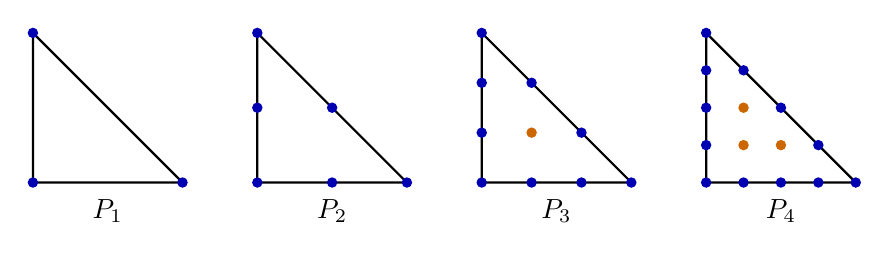
\begin{tikzpicture}[scale=1.9]
\foreach \p/\xo in {1/0,2/1.5,3/3,4/4.5} {
  \begin{scope}[shift={(\xo,0)}]
  \draw[thick] (0,0) -- (1,0) -- (0,1) -- cycle;
  \pgfmathtruncatemacro{\pp}{\p}
  \foreach \a in {0,...,\pp} {
    \pgfmathtruncatemacro{\bmax}{\pp-\a}
    \foreach \b in {0,...,\bmax} {
      \pgfmathsetmacro{\xx}{\a/\pp}
      \pgfmathsetmacro{\yy}{\b/\pp}
      \pgfmathtruncatemacro{\interior}{(\a>0)&&(\b>0)&&(\a+\b<\pp)}
      \ifnum\interior=1
        \fill[orange!80!black] (\xx,\yy) circle (0.035);
      \else
        \fill[blue!70!black] (\xx,\yy) circle (0.035);
      \fi
    }
  }
  \node[below] at (0.5,-0.05) {$P_{\p}$};
  \end{scope}
}
\end{tikzpicture}
\caption{参考三角形上 $P_1$ 到 $P_4$ 的节点 $\alpha/p$。蓝点在边界上，橙点在内部。局部基函数个数分别为 3、6、10、15。}
\label{fig:nodes}
\end{figure}

一般地，$p$ 次元的节点是所有形如
\[
\Bigl(\frac{\alpha_1}{p},\frac{\alpha_2}{p},\frac{\alpha_3}{p}\Bigr)\quad(\text{重心坐标}),\qquad \alpha_1,\alpha_2,\alpha_3\ \text{为非负整数},\ \alpha_1+\alpha_2+\alpha_3=p
\]
的点（图~\ref{fig:nodes}）。这样的 $\alpha$ 一共有 $\binom{p+2}{2}=\frac{(p+1)(p+2)}2$ 个：$p=2,3,4$ 时分别为 6、10、15，恰好等于二元 $p$ 次多项式空间的维数。对每个节点 $\alpha$，定义
\begin{equation}
\label{eq:lagrange}
N_\alpha(\lambda)=\prod_{i=1}^3\ \prod_{j=0}^{\alpha_i-1}\frac{p\lambda_i-j}{j+1}
\end{equation}
（若 $\alpha_i=0$，对应的内层乘积是空积，取为 1）。

\begin{proposition}
$N_\alpha$ 是 $p$ 次多项式，在节点 $\alpha$ 处取值 1，在其余节点处取值 0。
\end{proposition}

\begin{proof}
每个因子 $p\lambda_i-j$ 是一次的，共有 $\alpha_1+\alpha_2+\alpha_3=p$ 个因子，所以 $N_\alpha$ 是 $p$ 次多项式。

在节点 $\gamma$ 处，$p\lambda_i=\gamma_i$，因此
\[
N_\alpha=\prod_{i=1}^3\ \prod_{j=0}^{\alpha_i-1}\frac{\gamma_i-j}{j+1}.
\]
若某个 $i$ 有 $\gamma_i<\alpha_i$，则 $j=\gamma_i$ 出现在内层乘积中，因子 $\gamma_i-\gamma_i=0$，乘积为零。否则对所有 $i$ 都有 $\gamma_i\ge\alpha_i$；但 $\sum\gamma_i=\sum\alpha_i=p$，只能 $\gamma=\alpha$。此时内层乘积为 $\prod_{j=0}^{\alpha_i-1}\frac{\alpha_i-j}{j+1}=\frac{\alpha_i!}{\alpha_i!}=1$。
\end{proof}

由此，任意 $p$ 次多项式 $q$ 都可以写成 $q=\sum_\alpha q(\text{节点 }\alpha)\,N_\alpha$：两边都是 $p$ 次多项式，并且在所有节点上相等；而一个 $p$ 次多项式由它在这些节点上的值唯一确定（节点数等于空间维数，且上面的命题说明 $N_\alpha$ 线性无关）。所以有限元的未知数就是函数在节点上的值，称为\emph{自由度}。

\subsection{单元之间的连续拼接}
\label{sec:continuity}

在边 $\lambda_3=0$ 上，$p$ 次多项式限制为沿边参数的一元 $p$ 次多项式，它由这条边上的 $p+1$ 个节点值唯一确定。两个相邻三角形共享一条边及其上的 $p+1$ 个节点；只要它们在这些节点上取相同的值，两侧多项式在整条边上就完全相同。于是拼起来的函数是连续的，属于 $H^1$。

实现时有一个细节：同一条边在两个三角形中的局部方向可能相反。若在一个三角形中，这条边上的内部节点从一端数起依次编号为 $1,\dots,p-1$，在另一个三角形中同一节点的编号就是 $p-j$。只要按全局顶点编号统一边的方向，就能保证两侧对应同一个全局自由度。

每个三角形的 $\frac{(p+1)(p+2)}2$ 个局部自由度分为三类：3 个在顶点上（与周围所有三角形共享）；每条边上 $p-1$ 个（与相邻三角形共享）；内部 $\frac{(p-1)(p-2)}2$ 个（只属于这个三角形）。$p=4$ 时分别为 3、9、3 个。

\begin{keypoint}
同一网格上，$p$ 次多项式一定也是 $p+1$ 次多项式。因此几何不变时，$P_2$、$P_3$、$P_4$ 有限元空间是嵌套的：$V_2\subset V_3\subset V_4$。主讲义的“富化”就是在这三个嵌套空间中依次求解。
\end{keypoint}

% ======================================================================
\section{从参考三角形到实际单元：直边与曲边映射}
\label{sec:mapping}

上一节的基函数定义在参考三角形 $\widehat K$ 上。实际网格中的每个三角形 $K$ 都由一个映射 $F_K:\widehat K\to K$ 给出，基函数通过“复合”搬到 $K$ 上：
\[
\psi(x)=\widehat N\bigl(F_K^{-1}(x)\bigr),
\]
其中 $\widehat N$ 是参考三角形上的某个 $N_\alpha$。实际计算从不需要显式写出 $F_K^{-1}$，所有积分都拉回到参考三角形上做。

\subsection{直边三角形：仿射映射}

设 $K$ 的顶点为 $\bm x_1,\bm x_2,\bm x_3$。映射
\[
F_K(\xi,\eta)=\bm x_1+(\bm x_2-\bm x_1)\,\xi+(\bm x_3-\bm x_1)\,\eta
\]
把参考三角形的三个顶点依次送到 $\bm x_1,\bm x_2,\bm x_3$。它的 Jacobi 矩阵
\[
J=\frac{\partial(x,y)}{\partial(\xi,\eta)}=\bigl[\bm x_2-\bm x_1\ \big|\ \bm x_3-\bm x_1\bigr]
\]
是常数矩阵，$|\det J|$ 等于 $K$ 面积的两倍。

\subsection{积分与梯度的换元}

设 $\widehat f=f\circ F_K$ 表示把函数拉回到参考三角形。由二重积分换元公式，
\begin{equation}
\label{eq:change-var}
\int_K f\,\dd x=\int_{\widehat K}\widehat f(\xi,\eta)\,|\det J(\xi,\eta)|\,\dd\xi\,\dd\eta .
\end{equation}
梯度用链式法则。若 $\psi=\widehat N\circ F_K^{-1}$，则 $\widehat N(\xi,\eta)=\psi(F_K(\xi,\eta))$，对 $\xi,\eta$ 求导：
\[
\begin{pmatrix}\partial_\xi\widehat N\\ \partial_\eta\widehat N\end{pmatrix}
=J^{\mathsf T}\begin{pmatrix}\partial_x\psi\\ \partial_y\psi\end{pmatrix}
\quad\Longrightarrow\quad
\nabla\psi=J^{-\mathsf T}\,\widehat\nabla\widehat N ,
\]
其中 $\widehat\nabla=(\partial_\xi,\partial_\eta)^{\mathsf T}$。于是单元刚度矩阵的一个元素为
\begin{equation}
\label{eq:local-K}
\int_K\nabla\psi_b\cdot\nabla\overline{\psi_a}\,\dd x
=\int_{\widehat K}\bigl(J^{-\mathsf T}\widehat\nabla\widehat N_b\bigr)\cdot\bigl(J^{-\mathsf T}\widehat\nabla\widehat N_a\bigr)\,|\det J|\,\dd\xi\,\dd\eta .
\end{equation}
（实基函数不需要共轭；复数只来自后面的准周期约束。）这里 $a,b$ 是单元内的局部编号。

\subsection{为什么需要曲边单元}

材料界面是光滑曲线。若用直边三角形逼近一个圆，弦与弧之间的距离是 $O(h^2)$（$h$ 为边长）。这一几何误差会直接进入特征值，并且不随多项式次数 $p$ 的提高而减小：无论场用多高次的多项式，材料边界本身就画错了。

一个常用的改进是\emph{二次曲边单元}：每条边上除两个端点外再取一个“中点”，界面上的边把中点放在真实曲线上；然后用 $P_2$ 基函数插值几何，
\begin{equation}
\label{eq:p2-map}
F_K(\xi,\eta)=\sum_{i=1}^6\bm x_i\,\widehat N^{(2)}_i(\xi,\eta),
\end{equation}
其中 $\bm x_1,\dots,\bm x_6$ 是三个顶点和三个边中点，$\widehat N^{(2)}_i$ 是第~\ref{sec:lagrange}~节的六个二次基函数。这时每条界面边变成一段抛物线，它过真实曲线上的三个点，与真实曲线的距离降为 $O(h^3)$。

曲边单元带来三个变化：
\begin{enumerate}
\item $J$ 不再是常数，而是 $(\xi,\eta)$ 的一次函数，$\det J$ 是二次多项式。必须检查 $\det J$ 在整个单元上保持正号（映射不“翻转”），并且其最大值与最小值之比不太大。主讲义的数值实验报告了这个比值。
\item 公式 \eqref{eq:local-K} 中出现 $J^{-1}=\operatorname{adj}(J)/\det J$，被积函数含有 $1/\det J$，不再是多项式，所以数值积分不再精确（见第~\ref{sec:quad}~节）。
\item 相邻单元的共享边由同样三个几何节点定义，两侧映射在这条边上一致。因此第~\ref{sec:continuity}~节的连续性论证照样成立。
\end{enumerate}

\begin{keypoint}
主讲义中，几何始终用二次曲边映射，场的多项式次数 $p=2,3,4$。同一套映射下，$p$ 次函数也是 $p+1$ 次函数，嵌套关系 $V_2\subset V_3\subset V_4$ 仍然成立。但二次曲边只是\emph{近似}真实界面，两者之间夹着一条很薄的带。主讲义第~5~节专门处理这条薄带带来的材料误差。
\end{keypoint}

% ======================================================================
\section{数值积分}
\label{sec:quad}

刚度矩阵和质量矩阵的每个元素都是参考三角形上的积分，需要数值计算。

\subsection{一维 Gauss--Legendre 公式}

在 $[-1,1]$ 上，$m$ 点 Gauss--Legendre 公式
\[
\int_{-1}^1 g(s)\,\dd s\approx\sum_{q=1}^m w_q\,g(s_q)
\]
对所有次数 $\le 2m-1$ 的多项式精确成立。节点 $s_q$ 是 $m$ 次 Legendre 多项式的零点。例如 $m=2$ 时 $s_q=\pm1/\sqrt3$，$w_q=1$。可以直接验证：$g=s^2$ 时左边为 $2/3$，右边为 $2\cdot\frac13=\frac23$；$g=s^3$ 时两边都为零。

实际计算中，节点和权重可以由一个对称三对角矩阵的特征值和特征向量得到（Golub--Welsch 算法），这比求多项式零点稳定得多。变换 $s\mapsto(s+1)/2$ 把公式移到 $[0,1]$ 上，权重相应除以 2。

\subsection{正方形与三角形：Duffy 变换}

正方形 $[0,1]^2$ 上取两个方向的 Gauss 公式做张量积即可。三角形可以通过 \emph{Duffy 变换}化为正方形：
\[
\xi=r,\qquad \eta=(1-r)\,s,\qquad (r,s)\in[0,1]^2 .
\]
它把正方形的边 $r=1$ 压缩为三角形的顶点 $(1,0)$。它的 Jacobi 行列式为
\[
\det\frac{\partial(\xi,\eta)}{\partial(r,s)}=\det\begin{pmatrix}1&0\\-s&1-r\end{pmatrix}=1-r ,
\]
所以
\[
\int_{\widehat K}g(\xi,\eta)\,\dd\xi\,\dd\eta=\int_0^1\!\!\int_0^1 g\bigl(r,(1-r)s\bigr)\,(1-r)\,\dd r\,\dd s .
\]
右端两个方向各用 $m$ 点 Gauss 公式，得到三角形上的 $m^2$ 点公式。主讲义的数值实验中，“体积积分阶 12”就是 $m=12$，每个三角形 $144$ 个点。

若 $g$ 是 $(\xi,\eta)$ 的 $n$ 次多项式，则右端被积函数关于 $r$ 的次数不超过 $n+1$，关于 $s$ 的次数不超过 $n$。因此只要 $2m-1\ge n+1$，公式就是精确的。直边单元上 $P_4$ 质量矩阵的被积函数是 $8$ 次多项式，$m=5$ 已经足够。

\subsection{曲边单元上的积分误差}

曲边单元上，式 \eqref{eq:local-K} 的被积函数含 $1/\det J$，不是多项式，任何固定点数的公式都只能近似。由于 $\det J$ 在单元上变化不大（最大最小值之比接近 1），被积函数非常光滑，Gauss 公式收敛很快。

主讲义采用的做法是：用两套点数不同的公式（“主公式”与“检查公式”）各算一遍，比较结果。如果两次得到的特征值之差远小于关心的精度，就认为积分误差已经可以忽略。这是一个经验检查，不是严格界。

% ======================================================================
\section{组装}
\label{sec:assembly}

\subsection{局部矩阵与全局编号}

一个基函数只在包含它的节点的少数几个单元上非零，所以积分 $K_{ij}=\int\nabla\psi_j\cdot\nabla\overline{\psi_i}$ 可以拆成单元上的积分之和：
\[
K_{ij}=\sum_{K}\int_K\nabla\psi_j\cdot\nabla\overline{\psi_i}\,\dd x .
\]
每个单元有 $n_{\rm loc}=\frac{(p+1)(p+2)}2$ 个局部基函数。对每个单元算出 $n_{\rm loc}\times n_{\rm loc}$ 的\emph{局部矩阵}，再按“局部编号 $\to$ 全局编号”的对应关系累加到全局矩阵中。这个过程叫\emph{组装}。全局矩阵中绝大多数元素为零，用稀疏格式存储。

\begin{example}
一维 $P_1$ 元，单元 $[x_{j},x_{j+1}]$ 上两个局部基函数的局部刚度矩阵为
\[
\frac1h\begin{pmatrix}1&-1\\-1&1\end{pmatrix}.
\]
节点 $x_j$ 同时属于 $[x_{j-1},x_j]$ 和 $[x_j,x_{j+1}]$，两次累加后对角元为 $\frac1h+\frac1h=\frac2h$，与第~\ref{sec:hat}~节的直接计算一致。
\end{example}

\subsection{分片常数材料}

质量矩阵中有材料系数 $\rho$。网格生成时，每个三角形被标记为“在某个夹杂内部”或“在背景中”，$\rho$ 在每个单元上取常数。单元局部质量矩阵就是 $\rho_K\int_K\psi_b\overline{\psi_a}$。

注意：这样定义的材料实际上以\emph{网格的}曲边界面为分界线，而不是以真实界面为分界线。我们把它称为\emph{名义材料}。真实材料与名义材料只在一条薄带上不同，主讲义第~5~节给出修正方法。

% ======================================================================
\section{准周期约束}
\label{sec:qp-constraint}

第~\ref{sec:qp-weak}~节说明，函数空间中的函数要满足 $u(x,\tfrac12)=\ee^{\ii\beta}u(x,-\tfrac12)$。离散时，网格在上下边界上的节点一一对应（同一 $x$ 坐标），我们要求
\[
u(\text{上边界节点})=\ee^{\ii\beta}\,u(\text{对应的下边界节点}).
\]
上边界节点的值因此不是独立的未知量。

\subsection{约束矩阵}

记全部节点值组成的向量为 $\bm c_{\rm all}$，去掉上边界节点后剩下的“自由”节点值为 $\bm c$。定义稀疏矩阵 $Q$，使 $\bm c_{\rm all}=Q\bm c$：
\begin{itemize}
\item 对非上边界节点，$Q$ 的这一行在它自己的列上为 1；
\item 对上边界节点，$Q$ 的这一行在对应下边界节点的列上为 $\ee^{\ii\beta}$。
\end{itemize}
$Q$ 的每一行恰有一个非零元。

\subsection{约化后的矩阵}

在约束空间中，试探函数为 $Q\bm c$，测试函数为 $Q\bm w$，$\bm w$ 任意。Galerkin 方程变为
\[
\bm w^*Q^*K_{\rm all}Q\bm c=\mu\,\bm w^*Q^*M_{\rm all}Q\bm c\qquad\text{对所有 }\bm w ,
\]
即
\[
K\bm c=\mu M\bm c,\qquad K=Q^*K_{\rm all}Q,\qquad M=Q^*M_{\rm all}Q .
\]
由于 $K_{\rm all}$ 和 $M_{\rm all}$ 是实对称的，$K$ 和 $M$ 是 Hermite 的，$M$ 仍然正定。

\begin{example}
只看一对节点：下边界节点 $b$ 与上边界节点 $t$。设 $\bm c_{\rm all}=(c_b,c_t)^{\mathsf T}=(1,\ee^{\ii\beta})^{\mathsf T}c_b$，即 $Q=(1,\ee^{\ii\beta})^{\mathsf T}$。则
\[
K=Q^*K_{\rm all}Q=K_{bb}+\ee^{\ii\beta}K_{bt}+\ee^{-\ii\beta}K_{tb}+K_{tt}.
\]
$\beta=0$ 时这就是周期边界条件下把两个节点“粘起来”。$\beta\ne0$ 时出现复相位，矩阵变为复 Hermite 矩阵。
\end{example}

\subsection{竖直墙上的自由度}

主讲义经常要用到某条竖直线 $x=\text{常数}$（称为\emph{墙}）上的节点。假设网格在墙上有 $s$ 条边，那么墙上共有 $sp+1$ 个 $P_p$ 节点，其中最上面一个是上边界节点，被约束消去。所以每条墙上恰有 $sp$ 个自由度。主讲义的实验中 $s=48$，$P_2$、$P_3$、$P_4$ 每条墙分别有 96、144、192 个自由度。

墙上的有限元函数是一元分段 $p$ 次多项式（再加准周期闭合），它的“一维质量矩阵”
\[
W_{ij}=\int_{-1/2}^{1/2}\phi_j(y)\,\overline{\phi_i(y)}\,\dd y
\]
（$\phi_i$ 是墙上自由度对应的一维基函数）满足 $\bm g^*W\bm g=\int|g|^2\,\dd y$。主讲义用它来度量墙上迹的大小。

% ======================================================================
\section{静态凝聚：把一个单胞压缩到它的两面墙上}
\label{sec:schur}

这一节是理解主讲义中 DtN 方法的关键。

\subsection{动机}

主讲义要处理的区域是一条无限长的波导，由无穷多个单胞（宽度为一个周期的竖条）组成。我们不可能在整个无限区域上做有限元，但可以先把每个单胞内部的未知量“消去”，只留下单胞左右两面墙上的未知量。单胞之间只通过墙相互作用，所以消去内部之后，问题就只剩下墙上的未知量。这一思路在周期介质中的系统发展见 \cite{JolyLiFliss2006,Fliss2013}。

\subsection{分块与消元}

固定 $\mu$，记 $A=A(\mu)=K-\mu M$，它是 Hermite 矩阵（$\mu$ 为实数）。把一个单胞的自由度分为两类：墙上的（记为 $\Gamma$）和内部的（记为 $I$）。按这个顺序分块：
\[
A=\begin{pmatrix}A_{\Gamma\Gamma}&A_{\Gamma I}\\ A_{I\Gamma}&A_{II}\end{pmatrix}.
\]
考虑这样一个问题：给定墙上的值 $\bm g$，求内部的值 $\bm u_I$，使得有限元方程在所有\emph{内部}测试函数上成立。这正是第 $I$ 块行：
\[
A_{I\Gamma}\bm g+A_{II}\bm u_I=0\quad\Longrightarrow\quad\bm u_I=-A_{II}^{-1}A_{I\Gamma}\bm g .
\]
（需要 $A_{II}$ 可逆，见下文。）这样得到的函数称为 $\bm g$ 的\emph{离散延拓}，记
\begin{equation}
\label{eq:ext}
E\bm g=\begin{pmatrix}\bm g\\ -A_{II}^{-1}A_{I\Gamma}\bm g\end{pmatrix}.
\end{equation}
把它代入第 $\Gamma$ 块行，得到墙上的“剩余载荷”
\[
A_{\Gamma\Gamma}\bm g+A_{\Gamma I}\bm u_I=S\bm g,\qquad
S=A_{\Gamma\Gamma}-A_{\Gamma I}A_{II}^{-1}A_{I\Gamma}.
\]
矩阵 $S$ 称为 $A$ 关于内部块的 \emph{Schur 补}。

\emph{物理意义。} 在连续问题中，给定墙上的值，在单胞内解方程 $-\Delta u=\mu\rho u$，再取墙上的法向导数，这个映射叫做 Dirichlet-to-Neumann（DtN）映射。$S$ 正是它的离散版本：输入墙上的值，输出墙上的“载荷”（离散的法向导数，已经乘了测试函数积分）。

\begin{example}
一维 $P_1$ 元，三个节点 $0,h,2h$，取 $\mu=0$。两端是“墙”，中间是内部。$A=\frac1h\begin{pmatrix}1&-1&0\\-1&2&-1\\0&-1&1\end{pmatrix}$。按（左墙、右墙；内部）分块：
\[
A_{\Gamma\Gamma}=\frac1h\begin{pmatrix}1&0\\0&1\end{pmatrix},\quad
A_{\Gamma I}=\frac1h\begin{pmatrix}-1\\-1\end{pmatrix},\quad A_{II}=\frac2h ,
\]
\[
S=\frac1h\begin{pmatrix}1&0\\0&1\end{pmatrix}-\frac1h\begin{pmatrix}-1\\-1\end{pmatrix}\frac h2\cdot\frac1h\begin{pmatrix}-1&-1\end{pmatrix}
=\frac{1}{2h}\begin{pmatrix}1&-1\\-1&1\end{pmatrix}.
\]
这恰好是长度为 $2h$ 的单个单元的刚度矩阵：消去中点后，两段串联等价于一段长单元。
\end{example}

\subsection{能量恒等式}

设 $\bm u=E\bm g$。因为 $A\bm u$ 的内部块为零、墙块为 $S\bm g$，即 $AE\bm g=\binom{S\bm g}{0}$，所以
\begin{equation}
\label{eq:schur-energy}
\bm g^*S\bm g=\bm u^*A\bm u=\int_{\text{单胞}}|\nabla u|^2-\mu\int_{\text{单胞}}\rho|u|^2 ,
\end{equation}
其中 $u$ 是系数 $\bm u$ 对应的有限元函数。这说明 $S=E^*AE$，从而 $S$ 是 Hermite 矩阵。

\subsection{\texorpdfstring{Schur 补对 $\mu$ 的导数}{Schur 补对 mu 的导数}}
\label{sec:schur-deriv}

主讲义需要 $S(\mu)$ 对 $\mu$ 的导数。由 $S=E^*AE$ 和乘积法则，
\[
S'=(E')^*AE+E^*A'E+E^*AE' .
\]
$E$ 的上块是单位阵，与 $\mu$ 无关，所以 $E'$ 的上块为零：$E'=\binom{0}{\ast}$。又 $AE=\binom{S}{0}$，于是
\[
(E')^*AE=\begin{pmatrix}0&\ast^*\end{pmatrix}\begin{pmatrix}S\\0\end{pmatrix}=0 ,
\]
同理 $E^*AE'=(AE)^*E'=0$（这里用了 $A^*=A$）。最后 $A'=-M$，所以
\begin{equation}
\label{eq:schur-deriv}
S'(\mu)=-E^*ME,\qquad \bm g^*S'\bm g=-\int_{\text{单胞}}\rho\,|u|^2 .
\end{equation}
也就是说，Schur 补的导数等于负的“延拓函数的质量”。这个简单事实是主讲义第~6~节“导数等于无限质量”的单胞版本。

\subsection{\texorpdfstring{何时 $A_{II}$ 可逆}{何时内部块可逆}}

$A_{II}=K_{II}-\mu M_{II}$ 对应“墙上取零值”的单胞问题。它奇异，当且仅当 $\mu$ 恰好是这个问题（墙上 Dirichlet 条件、上下准周期条件）的离散特征值。主讲义中给出了中心单胞在关心的 $\mu$ 附近不会出现这种情形的理由；对侧向单胞，数值上检查条件数。

% ======================================================================
\section{嵌套的多项式空间与延拓矩阵}
\label{sec:nested}

同一网格、同一几何映射下，$V_p\subset V_{p+1}$。具体地说，$V_p$ 中的函数 $u$ 也可以用 $V_{p+1}$ 的基表示，系数就是 $u$ 在 $P_{p+1}$ 节点上的值（第~\ref{sec:pp}~节）。把这个关系写成矩阵：
\[
\bm c_{p+1}=J\bm c_p ,
\]
其中 $J$ 的第 $(i,j)$ 元是第 $j$ 个 $P_p$ 基函数在第 $i$ 个 $P_{p+1}$ 节点上的值。（准周期约束与 $J$ 相容，因为上下边界节点在两个空间中以同样方式配对。）

因为同一个函数的积分与用哪组基表示无关，
\[
\bm c_p^*K_p\bm c_p=\int|\nabla u|^2=\bm c_{p+1}^*K_{p+1}\bm c_{p+1}=\bm c_p^*J^*K_{p+1}J\bm c_p ,
\]
并且由极化恒等式，这对二次型成立就对矩阵成立：
\begin{equation}
\label{eq:nested}
K_p=J^*K_{p+1}J,\qquad M_p=J^*M_{p+1}J .
\end{equation}
数值上，只要两次组装用同一个积分公式，这两个等式就在舍入误差内成立。主讲义用它作为一个实现检查：如果 \eqref{eq:nested} 不成立，说明基函数或编号有错误。

主讲义还用到墙上的同类操作：把 $P_p$ 层求得的墙上迹（一维分段 $p$ 次多项式）在 $P_{p+1}$ 的墙节点上取值，作为下一层求根的初值。

% ======================================================================
\section{几个线性代数工具}
\label{sec:linalg}

\subsection{Hermite 广义特征值问题}

设 $K$ Hermite，$M$ Hermite 正定。对 $M$ 做 Cholesky 分解 $M=LL^*$（$L$ 是下三角矩阵），令 $\bm y=L^*\bm c$，则 $K\bm c=\mu M\bm c$ 化为标准 Hermite 特征值问题
\[
L^{-1}KL^{-*}\bm y=\mu\bm y .
\]
因此所有 $\mu$ 都是实数，特征向量可以取为关于 $M$ 正交：$\bm c_i^*M\bm c_j=\delta_{ij}$。

\subsection{特征值的导数（Hellmann--Feynman 公式）}
\label{sec:hf}

设 $F(\mu)$ 是依赖于实参数 $\mu$ 的 Hermite 矩阵，$W$ 是固定的 Hermite 正定矩阵。考虑广义特征值问题
\[
F(\mu)\bm g=\theta\,W\bm g ,
\]
设 $\theta(\mu)$ 是一个单重特征值，$\bm g(\mu)$ 是对应的特征向量，两者都光滑地依赖于 $\mu$。

\begin{proposition}
\label{prop:hf}
\[
\theta'(\mu)=\frac{\bm g^*F'(\mu)\bm g}{\bm g^*W\bm g}.
\]
\end{proposition}

\begin{proof}
对 $F\bm g=\theta W\bm g$ 关于 $\mu$ 求导：
\[
F'\bm g+F\bm g'=\theta'W\bm g+\theta W\bm g' .
\]
左乘 $\bm g^*$：
\[
\bm g^*F'\bm g+\bm g^*F\bm g'=\theta'\,\bm g^*W\bm g+\theta\,\bm g^*W\bm g' .
\]
因为 $F$ Hermite、$\theta$ 实，$\bm g^*F=(F\bm g)^*=(\theta W\bm g)^*=\theta\,\bm g^*W$，所以 $\bm g^*F\bm g'=\theta\,\bm g^*W\bm g'$，两边第二项相消，即得结论。
\end{proof}

注意，结论里不出现 $\bm g'$：特征值的一阶导数只需要特征向量本身，不需要知道特征向量怎样变化。

\emph{用于求根。} 若想找 $\mu$ 使 $\theta(\mu)=0$，Newton 法给出
\[
\mu_{\rm new}=\mu-\frac{\theta(\mu)}{\theta'(\mu)} .
\]
主讲义第~6~节用这一步从已知的近似特征值预测下一层的结果。实际求根时，我们用更稳健的“括号法”（保持 $\theta$ 在区间两端异号，用割线或 Brent 方法缩小区间）。

\subsection{二次特征值问题与线性化}
\label{sec:qep}

设 $A_2,A_1,A_0$ 是 $n\times n$ 矩阵。\emph{二次特征值问题}是：求数 $\zeta$ 和非零向量 $\bm v$，使
\begin{equation}
\label{eq:qep}
\bigl(\zeta^2A_2+\zeta A_1+A_0\bigr)\bm v=0 .
\end{equation}
令 $\bm z=\binom{\zeta\bm v}{\bm v}$，\eqref{eq:qep} 等价于 $2n$ 维的线性广义特征值问题
\begin{equation}
\label{eq:linearize}
\underbrace{\begin{pmatrix}-A_1&-A_0\\ I&0\end{pmatrix}}_{\mathcal A}\bm z=\zeta\underbrace{\begin{pmatrix}A_2&0\\0&I\end{pmatrix}}_{\mathcal B}\bm z .
\end{equation}
验证：第一块行是 $-A_1\zeta\bm v-A_0\bm v=\zeta A_2\zeta\bm v$，正是 \eqref{eq:qep}；第二块行是 $\zeta\bm v=\zeta\bm v$，恒成立。这个技巧叫\emph{线性化}，和把二阶常微分方程写成一阶方程组完全相同。它一共有 $2n$ 个特征值（$A_2$ 奇异时，其中一些是“无穷大”）。

\subsection{QZ 分解与不变子空间}
\label{sec:qz}

对广义特征值问题 $\mathcal A\bm z=\zeta\mathcal B\bm z$，数值稳定的标准算法是 \emph{QZ 分解}：存在酉矩阵 $\mathcal Q,\mathcal Z$，使
\[
\mathcal Q^*\mathcal A\mathcal Z=R_A,\qquad \mathcal Q^*\mathcal B\mathcal Z=R_B
\]
都是上三角矩阵。特征值是对角元之比 $(R_A)_{ii}/(R_B)_{ii}$。$(R_B)_{ii}=0$ 对应无穷大特征值，这在 QZ 中不造成任何困难，这是它比“先求 $\mathcal B^{-1}$”好的地方。

QZ 分解可以\emph{重新排序}（MATLAB 的 \texttt{ordqz}），把我们想要的特征值（例如所有满足 $|\zeta|<1$ 的）移到左上角。设排序后左上角有 $n$ 个特征值，取 $\mathcal Z$ 的前 $n$ 列 $Z_s$，$R_A,R_B$ 的左上 $n\times n$ 块为 $R_A^{11},R_B^{11}$。由 $\mathcal A\mathcal Z=\mathcal QR_A$ 的前 $n$ 列（上三角矩阵的前 $n$ 列只在前 $n$ 行非零）得
\[
\mathcal AZ_s=\mathcal Q_sR_A^{11},\qquad \mathcal BZ_s=\mathcal Q_sR_B^{11},
\]
其中 $\mathcal Q_s$ 是 $\mathcal Q$ 的前 $n$ 列。若 $R_B^{11}$ 可逆，消去 $\mathcal Q_s$：
\begin{equation}
\label{eq:deflating}
\mathcal AZ_s=\mathcal BZ_sT_s,\qquad T_s=(R_B^{11})^{-1}R_A^{11}.
\end{equation}
$T_s$ 是 $n\times n$ 上三角矩阵，它的特征值就是选出的那 $n$ 个 $\zeta$。$Z_s$ 的列张成的子空间叫做对应于这些特征值的\emph{紧缩子空间}。

\begin{proposition}
\label{prop:matrix-quadratic}
把 $Z_s$ 按 \eqref{eq:linearize} 的分块写成 $Z_s=\binom{Z_1}{Z_0}$。若 $Z_0$ 可逆，令 $T=Z_1Z_0^{-1}$，则
\[
A_2T^2+A_1T+A_0=0 ,
\]
并且 $T$ 的特征值恰好是选出的 $n$ 个 $\zeta$。
\end{proposition}

\begin{proof}
把 \eqref{eq:deflating} 按块写出。第二块行：$Z_1=Z_0T_s$，所以 $T=Z_0T_sZ_0^{-1}$，它与 $T_s$ 相似，特征值相同。并且 $Z_1=TZ_0$。

第一块行：$-A_1Z_1-A_0Z_0=A_2Z_1T_s$。其中
\[
Z_1T_s=TZ_0T_s=TZ_1=T^2Z_0 .
\]
代入得 $-A_1TZ_0-A_0Z_0=A_2T^2Z_0$。右乘 $Z_0^{-1}$ 即得结论。
\end{proof}

$T$ 称为矩阵二次方程的一个\emph{解}（solvent）。主讲义中，$T$ 描述“从一个单胞的墙走到下一个单胞的墙，场如何变化”；选择 $|\zeta|<1$ 的特征值意味着场在远离中心时衰减。

\subsection{Stein 方程与倍增算法}
\label{sec:stein}

设 $T$ 的所有特征值的模都小于 1，$C$ 是 Hermite 矩阵。\emph{Stein 方程}是
\begin{equation}
\label{eq:stein}
X-T^*XT=C .
\end{equation}

\begin{proposition}
\label{prop:stein}
\eqref{eq:stein} 的唯一解是
\[
X=\sum_{j=0}^\infty(T^*)^jC\,T^j .
\]
\end{proposition}

\begin{proof}
特征值的模都小于 1 时，$\|T^j\|$ 按几何级数趋于零，级数收敛。代入验证：
\[
T^*XT=\sum_{j=0}^\infty(T^*)^{j+1}C\,T^{j+1}=\sum_{j=1}^\infty(T^*)^jC\,T^j=X-C .
\]
唯一性：若 $Y-T^*YT=0$，反复代入得 $Y=(T^*)^jYT^j\to0$，所以 $Y=0$。
\end{proof}

若 $C$ 半正定，则 $X$ 半正定：$\bm g^*X\bm g=\sum_j(T^j\bm g)^*C(T^j\bm g)\ge0$。主讲义中，$\bm g^*X\bm g$ 就是一条半无限波导中所有单胞的质量之和。

\emph{倍增算法。} 直接逐项求和收敛很慢。倍增算法令 $X_0=C$，$Q_0=T$，并迭代
\[
X_{k+1}=X_k+Q_k^*X_kQ_k,\qquad Q_{k+1}=Q_k^2 .
\]
用归纳法可以验证 $Q_k=T^{2^k}$ 和
\[
X_k=\sum_{j=0}^{2^k-1}(T^*)^jC\,T^j :
\]
设它对 $k$ 成立，则
\[
Q_k^*X_kQ_k=\sum_{j=0}^{2^k-1}(T^*)^{j+2^k}C\,T^{j+2^k}=\sum_{j=2^k}^{2^{k+1}-1}(T^*)^jC\,T^j ,
\]
加上 $X_k$ 恰好是到 $2^{k+1}-1$ 的和。所以每做一步，求和的项数翻倍，$k$ 步就求和了 $2^k$ 项。

\emph{截断误差。} 剩余部分为 $X-X_k=\sum_{j\ge2^k}(T^*)^jCT^j=Q_k^*XQ_k$。记 $r=\|Q_k\|_2<1$，由 $\|AB\|_F\le\|A\|_2\|B\|_F$，
\[
\|X-X_k\|_F\le r^2\|X\|_F\le r^2\bigl(\|X_k\|_F+\|X-X_k\|_F\bigr)
\quad\Longrightarrow\quad
\|X-X_k\|_F\le\frac{r^2}{1-r^2}\,\|X_k\|_F .
\]
右端完全可以计算，因此可以作为停止判据。

\begin{keypoint}
本教程到此为止介绍的工具，在主讲义中的用法是：弱形式与 Galerkin（第~\ref{sec:weak}--\ref{sec:galerkin}~节）给出每个单胞上的矩阵；高阶曲边元、积分和准周期约束（第~\ref{sec:lagrange}--\ref{sec:qp-constraint}~节）把矩阵实际算出来；静态凝聚（第~\ref{sec:schur}~节）把单胞压缩到墙上；二次特征值问题和 QZ（第~\ref{sec:qep}--\ref{sec:qz}~节）处理半无限波导；Hellmann--Feynman 公式和 Stein 方程（第~\ref{sec:hf}、\ref{sec:stein}~节）给出特征值的导数，进而给出 Newton 预测。
\end{keypoint}

\bibliographystyle{plainnat}
\bibliography{references}

\end{document}
